\chapter{Requirements}\label{chap:requirements}

Understanding the foundation for what the system aims to achieve is essential for guiding development. The following chapter presents a structured overview of the project's intentions, including the goals it seeks to fulfill, the constraints it operates under, and the needs of its intended users. These requirements were gathered in collaboration with the product owner and refined to ensure clarity and feasibility. They include high-level objectives such as product, impact, and learning goals. In addition, the chapter outlines limitations, use cases, and considerations for universal design. Together, these elements define the scope, purpose, and direction of the project and form a basis for implementation, testing, and evaluation.

\begin{comment}
BRA: (fra discussion)
    This chapter presents a reflection on both the development process and the final product. It examines how the project evolved in relation to the original goals, highlighting what worked well, what could have been improved, and the challenges encountered along the way. The chapter discusses the choice of technologies, project management practices, and team collaboration. It also evaluates the effectiveness and limitations of the final solution, comparing it with existing alternatives and identifying unexpected findings. Broader considerations, such as sustainability and the role of AI in the project, are explored. Finally, the chapter outlines potential directions for future work and improvements to both the product and the project approach.
\end{comment}


\section{Project Goals}

This section outlines the overall goal of the project, categorized into \textbf{product goals}, \textbf{impact goals}, and \textbf{learning goals}. Together, these objectives defines the purpose, intended outcomes, and the knowledge expected to be gained through the project process.
\subsection{Product Goals}\label{subsec:req:productgoals}

The primary goal of the project is to develop and test a \textbf{prototype system for fully digital modeling of forestry road load-bearing capacity under varying conditions throughout the year.} 

The following goals were provided by the \Gls{productowner} (see \autoref{appendix:task_description}):
\begin{itemize}
    \item Develop the methodology for a fully digital classification of the load-bearing capacity of forestry roads.
    \item Integrate the methodology with existing forecasts for operating conditions throughout the year.
    \item Combine these into a simple map-based visualization of the trafficability of forestry roads.
\end{itemize}

While these goals establish a general direction, they are relatively high-level. To ensure a clear and focused development process, they have been expanded into a set of more concrete and actionable goals that cover both functional and nonfunctional aspects and guide the implementation and evaluation of the prototype: 

\textcolor{orange}{Burde man spesifisere hvilke som er functional og non-functional goals?}

\begin{enumerate}
    \item \textbf{Data Collection and Integration:}
    \begin{itemize}
        \item Gather relevant geological and meteorological data, including superficial deposits, soil moisture, groundwater, ground frost, and forestry roads.
        \item Identify and implement suitable data sources and APIs for continuous updates.
    \end{itemize}
    
    \item \textbf{Classification and Forecasting:}
    \begin{itemize}
        \item Develop a rule-based model to classify road conditions based on environmental factors. 
        \item Implement a traffic-light classification system
        \begin{itemize}
            \item Green = Safe
            \item Yellow = Caution
            \item Red = Unsafe
        \end{itemize}
        \item Extend the model to provide a forecast of road conditions at least one week in advance. 
    \end{itemize}
    
    \item \textbf{Web-Based Visual and User Interface:}
    \begin{itemize}
        \item Design and develop an interactive, map-based website for intuitive accessibility. 
        \item Implement a way to visualize historical and forecasted data relevant to road conditions.
        \item Ensure that the system is optimized for transport managers, with a user-friendly interface that enables efficient decision-making. 
    \end{itemize}
    
    \item \textbf{Testing, Validation and Refinement}:
    \begin{itemize}
        \item Evaluate the accuracy and usability of the system by testing with real-world data. 
        \item Conduct user testing with transport managers or forestry stakeholders to assess the effectiveness of the interactive interface and forecasting capabilities. 
        \item Incorporate potential user feedback. 
    \end{itemize} 
\end{enumerate}


\subsection{Impact Goals}\label{subsec:req:impactgoals}

The project aims to deliver real-world value by improving decision-making processes related to forestry road usage. The following impact goals outline the intended benefits for end-users and stakeholders:

\begin{itemize}
    \item Reduced uncertainty for transport managers when setting the routes using forestry roads.
    \item To validate the prototype as a proof of concept and evaluate its feasibility and effectiveness as a foundation for a future operational system in the forestry industry.
\end{itemize}

\subsection{Learning Goals}\label{subsec:req:learninggoals}

In addition to delivering a functional prototype, the project serves as a valuable learning experience. The goals below reflect the desired technical and professional growth for the project participants and are categorized into \textbf{technical goals} and \textbf{project management goals}.

\textbf{Technical Goals}
\begin{itemize}
    \item Gaining insight in implementing interactive maps and geospatial data on websites.
    \item Leveraging \acrshort{rest}ful \acrshort{api}s for efficient data integration.
    \item Enhancing application performance by implementing concurrency and optimizing parallel processing.
    \item Expanding proficiency in containerization techniques, particularly through hands-on experience with Docker.
\end{itemize}

\textbf{Project Management Goals}
\begin{itemize}
    \item Acquiring hands-on experience collaborating with real-world companies and products.
    \item Gaining experience working in a team environment, improving collaboration and communication skills.
    \item Conducting user tests and implementing feedback. 
    \item Developing a deeper understanding of the software development life cycle while actively practicing agile methodologies, like Scrum and Kanban.
\end{itemize}

\section{Limitations}

\textcolor{orange}{Kan kanskje kalles, "Scope". Da må man skrive både hva systemet er og hva det ikke er.}

Applikasjonen fokuserer på norge og er på norsk. For å utvide måtte man ha brukt andre kilder i tilegg da, datakildene brukt er kun fra norge.

Klassifiseringen av veier går ut i fra at alle er konstruert med stedegne løsmasser, men dersom man får tilgang til veikonstruksjonsdata så kan man legge til dette som faktor (knust fjell -> sortert grus -> stedegne løsmasser).


\section{Constraints}

This project is subject to several constraints that have influenced the development process and final product. These include \textbf{temporal constraints} related to fixed academic deadlines and \textbf{product-related constraints} tied to technical and environmental requirements.

\subsection{Temporal Constraints}

The project must be completed within a limited timeframe due to university deadlines. These deadlines affect how much functionality and polish can reasonably be achieved.

\begin{itemize}
    \item The set deadline for the final thesis is the 20th of May.
    \item The presentation of the bachelor's thesis is scheduled for the 4th of June.
\end{itemize}

\subsection{Product Constraints}

The product is also subject to technical limitations that define the environment in which it must operate. These include requirements for connectivity, browser compatibility, and deployment conditions.

\begin{itemize}
    \item The product requires a stable network connection to be used.
    \item The product uses \acrshort{html} 5, which requires newer versions of browsers.
    \item The product needs to be deployed either locally or on a server to run.
\end{itemize}

\begin{comment}
    \subsection{Legal Constraints}
% VET IKKE OM DETTE SKAL VÆRE MED
% ENDRE TIL NÅTID (THE PRODUCT COMPLIES WITH....) ?
\begin{itemize}
    \item The product must comply with the licensing terms and conditions of all third-party services, including map distributors, external APIs, and any code libraries, frameworks, or tools used in its development and deployment.
\end{itemize}
\end{comment}

\section{Target Users}

The primary target users of this application are \textbf{transport managers in the Norwegian forestry industry}. They are responsible for planning routes and determining which forest roads should be used by drivers. The application is primarily intended to be used in an office setting during the planning phase. Since the user group spans a wide age range, it is essential that the application is intuitive and easy to use, ensuring accessibility for all users regardless of their technical proficiency.


\section{Use Case}

Use cases provide a clear overview of what a system will do. They enable effective scope management and incremental development, making them well-suited for agile methodologies \cite{jacobson_use_case}. 

This section will present the use case diagram of the system and provide an example of a use case specification.

\subsection{Use Case Diagram}
% DOBBELSJEKK AT SERVEREN IKKE SKAL KOBLES TIL USE CASENE I DIAGRAMMET
The use case diagram (\autoref{fig:use_case_diagram}) provides an overview of the system's core functionality by showing all user interactions with the website. It also depicts how the application server communicates with external map services.


\begin{figure}[h]
    \centering
    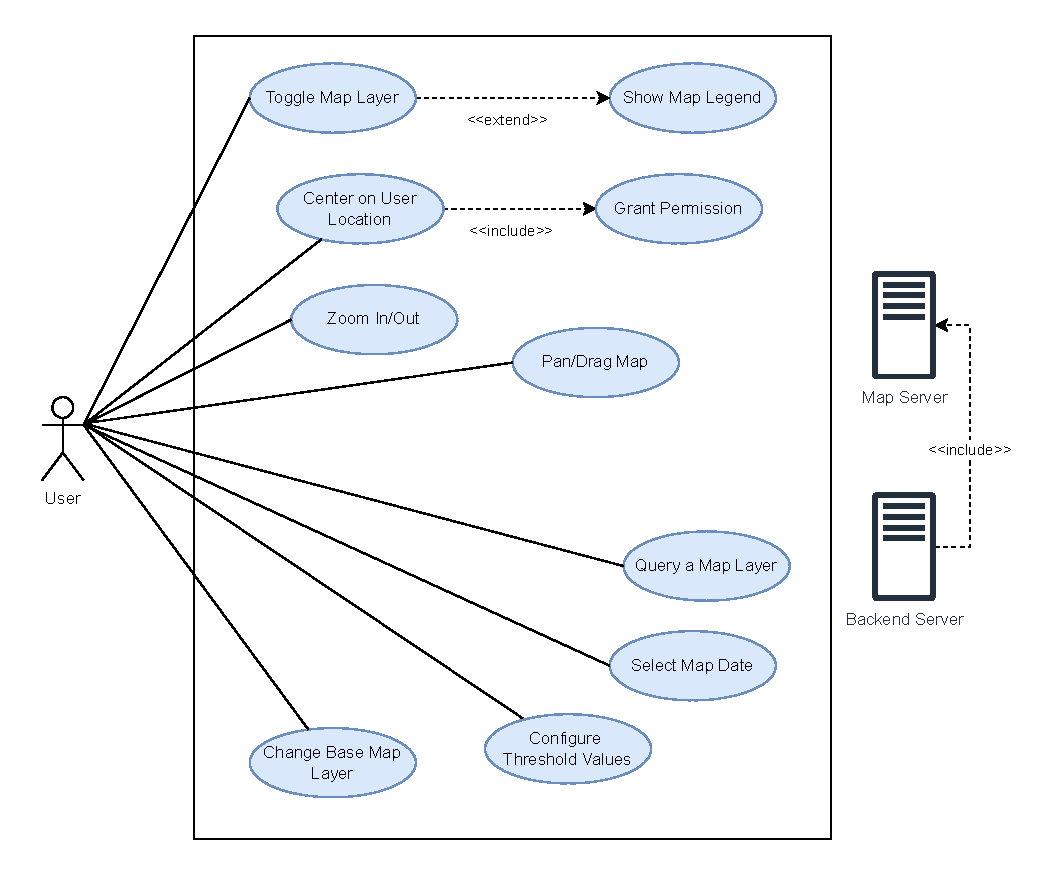
\includegraphics[width=1\linewidth]{figures/skogkurs_use_case.pdf}
    \caption{Use case diagram of system}
    \label{fig:use_case_diagram}
\end{figure}

\subsection{Actors}

\begin{itemize}
    \item \textbf{User:} The primary user of the website, typically transport managers in the Norwegian forestry industry, who interact with the system to access relevant map and logistics data.
    \item \textbf{Backend Server:} The central server that the website communicates with to retrieve all necessary map data. It aggregates, processes, and refines data from external services before delivering it to the website.
    \item \textbf{Map Server:} External services that provide map data, either through a Web Map Service (\Gls{wms}), Web Feature Service (\Gls{wfs}), or an \acrshort{api}. These services are integrated into the system by the backend server.
\end{itemize}

\subsection{Use Case Specifications}

It is important to show how users interact with the system to achieve their goals. The use case specifications provide details of each use case and the basic path the user takes to achieve their goals while also capturing possible exceptions. 

A high priority use case for the website is the ability to toggle a map layer, which allows users to control the visibility of different layers. The use case specification for this functionality is shown in \hyperref[tab:use_case_toggle_layer]{Table \ref*{tab:use_case_toggle_layer}}. Additional use case specifications for other features can be found in \hyperref[appendix:use_case_specifications]{Appendix \ref*{appendix:use_case_specifications}}.

\begin{table}[h]
    \centering
    \begin{tabularx}{\textwidth}{|l|X|}
        \hline
        \rowcolor{gray!20}
        \textbf{Use Case Name} & Toggle Map Layer \\
        \hline
        \textbf{Actor(s)} & User \\
        \hline
        \textbf{Description} & The user can toggle the visibility of individual map layers using checkboxes in the map layer menu. This allows users to control which layers are shown on the map, and relevant information about the visible layers is displayed in the legend sidebar. \\
        \hline
        \textbf{Priority} & High \\
        \hline
        \textbf{Pre-Condition(s)} & The user must have a stable internet connection and the website open. The website, server and external map servers must be deployed and running.\\
        \hline
        \textbf{Post-Condition(s)} & The selected map layer is displayed or hidden based on the user's input. The map legend updates accordingly in the legend sidebar. \\
        \hline
        \textbf{Basic Path} &  
        \begin{enumerate}[label=,left=0pt]
            \item 1. User connects to the website.
            \item 2. User presses the map layer ("kartlag") button to open the map layer sidebar.
            \item 3. User clicks the toggle button for the specific map layer to appear.
            \item 4. The system updates the map with the selected layer.
        \end{enumerate} \\
        \hline
        \textbf{Exception Path} & 
        \begin{enumerate}[label=,left=0pt]
            \item 1a. User does not have a stable internet connection and can not connect to the website.
            \item 3a. Either the backend server or the map server is not responding, and no map data is received.
        \end{enumerate} \\
        \hline
    \end{tabularx}
    \caption[Use Case Specification: Toggle Map Layer]{Use case for toggling a map layer}
    \label{tab:use_case_toggle_layer}
\end{table}

\section{Universal Design}

\begin{comment}
HVA ER WCAG
HVA ER UNIDES
UUtilsynet: https://www.uutilsynet.no/veiledning/introduksjon-til-universell-utforming/238
HVORFOR VI IKKE BRUKER DET/TATT HØYDE FOR DET
IKKE GJORT I PROTOTYPEN, MEN KAN BLI UTVIKLET SENERE I DISCUSSION
SKOGKURS = IKKE OFFENTLIG, OG PROTO = INGEN WCAG! :O

    JO HA MED DENNE
    Kanskje ikke nødvendig med eget kapittel og kanskje ha det et annet sted? Passer med overgang fra Target Audience ^. SIDEN NOE OM DETTE IKKE BLE NEVNT AV SKOGKURS SÅ BURDE DET KANSKJE STÅ I DISCUSSION I STEDET.

lovdata OM UU: https://lovdata.no/lov/2017-06-16-51/§17

Her skriver vi at:
SKogkurs ikke er statlig eid, produktet er ikke ment for allmineligheten,
produktet er en prototype.
Derfor er det ikke NØDVENDIG/KRAV om wcag/UU,
men vi vil gjerne ha det med for å styrke brukeropplevelsen
Så ikke stort fokus på det, men alle valg blir tatt med det i bakhaue
Funksjonalitete > uu
\end{comment}

Universal design refers to the practice of designing products, environments, and digital solutions in a way that ensures they can be used by as many people as possible, regardless of functional ability. The goal is not to create one solution for each user group, but rather to remove barriers so that everyone can use the same solution equally \cite{uutilsynet}.

In web development, universal design is often guided by the \acrfull{wcag}\footnote{\url{https://www.w3.org/WAI/standards-guidelines/wcag/}}, currently at version 2.2. These guidelines offer a broad set of recommendations aimed at making web content more accessible for people with a variety of disabilities, including visual, auditory, motor, and cognitive impairments. WCAG also promotes general usability, which often benefits all users, not just those with disabilities. It applies across platforms and devices, from desktops and laptops to smartphones and kiosks \cite{wcag}.

In Norway, the legal foundation for universal design is laid out in the Equality and Anti-Discrimination Act (Likestillings- og diskrimineringsloven), particularly in § 17–19a. These laws state that both public and private entities directed toward the general public are required to ensure their main solutions are universally designed. This includes digital solutions that are intended for users. However, the requirement does not apply if universal design would impose a disproportionate burden on the organization, considering factors such as cost, available resources, the nature of the business, and the potential benefits of removing accessibility barriers \cite{lovdata}.

\textbf{Rationale for Not Prioritizing Universal Design}

In this project, universal design was not a primary focus for several reasons. The prototype was developed on behalf of Skogkurs and the product is not aimed at the general population. As such, the legal requirement for universal design according to §17 and §18 in the law does not apply directly. Additionally, the product is still in a prototype phase and not in active use.

However, we recognize the importance of universal design in creating inclusive digital services. Although not implemented in the current version, accessibility and universal design considerations have been kept in mind throughout development. Our choices have prioritized functionality and technical feasibility, but without intentionally creating barriers for users with disabilities. We consider universal design an important area for future development and discuss potential improvements in \autoref{chap:discussion}.
